% !TeX root = thesis.tex
\documentclass[
    11pt,
    a4paper,
    egregdoesnotlikesansseriftitles,
    toc=chapterentrywithdots,
    twoside,openright,
    titlepage,
    parskip=half,
    headings=normal,  % reduces heading size
    listof=totoc,
    bibliography=totoc,
    index=totoc,
    captions=tableheading,  % caption below table
    % chapterprefix,
    listof=flat,
    final
]{scrbook}

% details about your thesis
\newcommand{\titel}{Entwicklung eines Suchalgorithmusprototyps zur Bewertung von Suchergebnissen verschiedener Kategorien}
\newcommand{\artderarbeit}{Studienarbeit}  % {Bachelorarbeit,Masterarbeit}
\newcommand{\autor}{Marc Jonas Roser}
\newcommand{\studiengang}{Software Engineering}  % {Informatik,Wirtschaftsinformatik,Medieninformatik}
\newcommand{\matrikelnr}{364\,7316}
\newcommand{\erstgutachter}{Prof.\,Dr.~Hans-Georg Hopf}
\newcommand{\zweitgutachter}{}
\newcommand{\betreuer}{}
\newcommand{\unternehmen}{}
\newcommand{\logo}{figures/TH-Nuernberg-RGB.png}
\newcommand{\keywords}{}
\newcommand{\publishDate}{06.10.2022}

% custom head and foot
\usepackage[automark]{scrlayer-scrpage}

\pagestyle{scrheadings}
\ihead{\headmark}
\chead{}
\ohead{\pagemark}
\renewcommand*\sectionmarkformat{
  \chapappifchapterprefix{\ }%
  \thechapter.\enskip
}

% Chapter and Section margins
% If needed adjust margins here to drastically increase pages ;)
\RedeclareSectionCommand[
  beforeskip=0\baselineskip,
  afterskip=.5\baselineskip]{chapter}
\RedeclareSectionCommand[
  tocindent=0pt,
  beforeskip=-.75\baselineskip,
  afterskip=.25\baselineskip]{section}
\RedeclareSectionCommand[
  tocindent=10pt,
  beforeskip=-.5\baselineskip,
  afterskip=.1\baselineskip]{subsection}

\usepackage{scrhack}

% other packages
\usepackage[utf8]{inputenc}
\usepackage[T1]{fontenc}
\usepackage{lmodern,relsize,textcomp,csquotes}
\usepackage{amsfonts}
\usepackage[english,ngerman]{babel}
\usepackage[english,ngerman]{tracklang}
\usepackage{caption}
\usepackage{subcaption}
% Label format
\DeclareCaptionLabelFormat{custom}
{%
  \textbf{#1 (#2)}
}
% Separator style
\DeclareCaptionLabelSeparator{custom}{--}
% Caption format
\DeclareCaptionFormat{custom}
{%
  #1#2\small #3
}
\captionsetup
{
  format=custom,%
  labelformat=custom,%
  labelsep=custom
}

\usepackage{graphicx}
\usepackage{wrapfig}
\usepackage{setspace,geometry,xcolor}
\usepackage{makeidx}
\usepackage{url}

\usepackage{pdfpages}

% table setup
\usepackage{longtable}
\usepackage{array}
\usepackage{ragged2e}
\usepackage{lscape}

\usepackage{listings}
\usepackage{xcolor}

\definecolor{codegreen}{rgb}{0,0.6,0}
\definecolor{codegray}{rgb}{0.5,0.5,0.5}
\definecolor{codepurple}{rgb}{0.58,0,0.82}
\definecolor{backcolour}{rgb}{0.95,0.95,0.92}
\lstdefinestyle{mystyle}{
    backgroundcolor=\color{backcolour},
    commentstyle=\color{codegreen},
    keywordstyle=\color{magenta},
    numberstyle=\tiny\color{codegray},
    stringstyle=\color{codepurple},
    basicstyle=\ttfamily\footnotesize,
    breakatwhitespace=false,
    breaklines=true,
    captionpos=b,
    keepspaces=true,
    numbers=left,
    numbersep=5pt,
    showspaces=false,
    showstringspaces=false,
    showtabs=false,
    tabsize=2
}
\lstset{
  style=mystyle,
  literate=% Allow for German characters in lstlistings.
  {Ö}{{\"O}}1
  {Ä}{{\"A}}1
  {Ü}{{\"U}}1
  {ß}{{\ss}}2
  {ü}{{\"u}}1
  {ä}{{\"a}}1
  {ö}{{\"o}}1
}
% pdf hyperref
\usepackage[
    bookmarks=true,
    bookmarksopen=true,
    bookmarksnumbered=true,
    bookmarksopenlevel=1,
    pdftitle={\titel},
    pdfauthor={\autor},
    pdfcreator={\autor},
    pdfsubject={\titel},
    pdfkeywords={\keywords},
    pdfpagelabels=true,
    colorlinks=true,
    linkcolor=black,
    urlcolor=magenta,
    anchorcolor=black,
    citecolor=cyan,
    filecolor=magenta,
    menucolor=red,
    plainpages=false,
    hypertexnames=true,
    linktocpage=true,
    linktoc=all,
    % hidelinks Uncomment in Production build
]{hyperref}
\usepackage[nonumberlist]{glossaries}

% page setup
% \setlength{\topskip}{\ht\strutbox}
\geometry{paper=a4paper,left=2.5cm,top=3.0cm,bindingoffset=.8cm}
\onehalfspacing
\frenchspacing
\clubpenalty = 10000
\widowpenalty = 10000
\displaywidowpenalty = 10000

% Uncomment to enable better printing support
% \clearpage
% Comment to enable better printing support
\let\cleardoublepage=\clearpage

% load glossary entries
\makenoidxglossaries
% \setglossarystyle{altlistgroup}
\setglossarystyle{altlist}
\loadglsentries{glossary}

% Remove hbox errors
\hfuzz=7.5pt

\begin{document}

\setcounter{secnumdepth}{3}  % numerate subsections
\setcounter{tocdepth}{2}  % ...but don't include them in toc

\frontmatter
\thispagestyle{empty}
\pagenumbering{Roman}
\thispagestyle{empty}
\pdfbookmark[1]{Cover}{cov}
\begin{titlepage}

\begin{center}

\includegraphics[width=\linewidth]{figures/TH-Nuernberg-RGB.png}\\[1cm]
\LARGE{Fakultät Elektrotechnik Feinwerktechnik Informationstechnik}\\[2cm]

\huge
\textbf{\titel}\\[1cm]
%
\Large
\artderarbeit~im Studiengang \studiengang\\[1cm]
%
\large
vorgelegt von

\Large
\autor\\[0.5cm]
\small
Matrikelnummer \matrikelnr\\[2cm]

\vspace*{\fill}

\large
\begin{tabular}{p{3cm}p{8cm}}\\
Erstgutachter:  & \quad \erstgutachter\\[1.2ex]
Zweitgutachter: & \quad \zweitgutachter\\[1.2ex]
%discomment "Betreuer" and "Unternehmen" for a thesis in a company
%Betreuer: & \quad \betreuer\\
%Unternehmen: & \quad \unternehmen
\end{tabular}
\end{center}

\begin{center}
\copyright\,\the\year
\end{center}

\vspace{-0.5cm}
\singlespacing
\small
\noindent Dieses Werk einschließlich seiner Teile ist \textbf{urheberrechtlich geschützt}.
Jede Verwertung außerhalb der engen Grenzen des Urheberrechtgesetzes ist ohne Zustimmung des Autors unzulässig und strafbar.
Das gilt insbesondere für Vervielfältigungen, Übersetzungen, Mikroverfilmungen sowie die Einspeicherung und Verarbeitung in elektronischen Systemen.

\end{titlepage}

\thispagestyle{empty}
\section*{Kurzdarstellung}
\label{sec:kurzdarstellung}
Das Ziel der vorliegenden Studienarbeit ist es, eine bestehende Datenbank mit multimedialen Inhalten möglichst effizient nach unterschiedlichen Kriterien zu durchsuchen.
Suchergebnisse sollen nach bestimmten Kriterien gewichtet, gefiltert und sortiert werden. Vorschläge für eine weiterführende Navigation auf der Suchergebnisseite sollen angeboten werden, Suchergebnisse sollen dazu nach Kontext und Wahrscheinlichkeiten gewichtet angezeigt werden.
Das theoretische Fundament dieser Arbeit stellt die wissenschaftliche Betrachtung der Methoden zur Bewertung der Relevanz von Suchergebnissen dar. Die Arbeit untersucht die Möglichkeit, einen Suchbegriff so zu analysieren, dass ein Nutzer die bestmögliche Ergebnisliste bzw. zielgerichtete weiterführende Navigationsmöglichkeiten erhält.
Die bestehende Anwendung "\gls{crossload}" wird vorgestellt, um dem Leser einen Kontext zu bieten, in der sich die Entwicklung bewegt.

\section*{Abstract}
\label{sec:abstract}
The goal of this student research project is to search an existing database with multimedia content as efficiently as possible according to various criteria.
Search results are to be weighted, filtered, and sorted according to certain criteria. Suggestions for further navigation on the search results page are to be offered, and search results are to be displayed weighted according to context and probabilities.
The theoretical foundation of this work is the scientific consideration of methods for evaluating the relevance of search results. The work examines the possibility of analyzing a search term in such a way that a user receives the best possible list of results or targeted further navigation options.
The existing application "Crossload" is presented to provide the reader with a context in which the development takes place.

\clearpage
\section*{Eidesstattliche Erklärung}
\label{sec:explanation}
Hiermit versichere ich, Marc Jonas Roser, ehrenwörtlich, dass ich die vorliegende Studienarbeit mit dem Titel: „Entwicklung eines Prototypen eines Suchalgorithmus zur Bewertung von Suchergebnissen verschiedener Kategorien“ selbstständig und ohne fremde Hilfe verfasst und keine anderen als die angegebenen Hilfsmittel benutzt habe. Die Stellen der Arbeit, die dem Wortlaut oder dem Sinn nach anderen Werken entnommen wurden, sind in jedem Fall unter Angabe der Quelle kenntlich gemacht. Die Arbeit ist noch nicht veröffentlicht oder in anderer Form als Prüfungsleistung vorgelegt worden.
Ich versichere zudem, dass die eingereichte elektronische Fassung mit der gedruckten Fassung übereinstimmt.

Nürnberg, 25.09.2022

Marc Jonas Roser

\printnoidxglossaries
\tableofcontents

\mainmatter
\chapter{Einleitung}\label{ch:intro}

\section{Relevanz des Themas}
Suchalgorithmen und relevante Suchergebnisse sind derzeit so relevant wie noch nie.
Dabei wollen die Benutzer einer Suchmaschine in Sekundenbruchteilen Ergebnisse, die am besten zu ihrem Suchbegriff passen, ohne sich dabei viel Gedanken über die Formulierung eines solchen Begriffes zu machen.
Ein Beispiel für einen solchen Algorithmus ist Google, welches seit den frühen 2000ern einen kometenhaften Aufstieg in der Welt der Suchmaschinen hinter sich hat, was anhand der erreichten Werbeeinnahmen sichtbar wird.\footnote{Siehe \ref{fig:werbeumsatz}}
Google ist im Vergleich zu anderen Suchmaschinen so stark verbreitet\footnote{Siehe \ref{fig:marketshare}}, dass mittlerweile sogar der Duden das Verb „googeln“ als eigenen Begriff für die Recherche im Internet führt.\footnote{Vgl. Duden \cite{duden2022}}
Dabei stellt sich für die Entwicklung eigener Produkte die Frage, wie aus einem Suchbegriff, der meist nur aus wenigen Wörtern bis zu einem ganzen Satz besteht, relevante Suchergebnisse gefunden werden können. Dies würde zur Akzeptanz der Nutzer im Hinblick auf die entwickelte Funktionalität führen, da gewünschte Ergebnisse schneller und ohne großen Aufwand gefunden werden können.

\section{Ausgangssituation}
Derzeit besteht bei \gls{crossload}\footnote{Siehe Crossload.org \cite{pfleiderer2022}}, einer Plattform zum Durchsuchen und Anhören einer umfassenden Predigt Datenbank, eine Datenbank mit einer Such \gls{api} auf Basis von Spring Boot und \gls{solr}. Diese teilt auf der Suchergebnisseite die Ergebnisse nach Kategorien auf und somit können nur schwer übergreifende Suchanfragen getätigt werden. Zwar werden alle Treffer auf der gleichen Seite angezeigt, doch durch die Aufteilung nach Kategorien werden Ergebnisse gewisser Kategorien über anderen gezeigt, auch wenn niedrig positionierte Kategorien relevantere Ergebnisse enthalten.

\section{Zielsetzung}
Das Ziel der vorliegenden Studienarbeit ist es durch eine theoretische Betrachtung der Bewertung der Relevanz von Suchergebnissen und der anschließenden Entwicklung eines Prototyps, ein bestehendes Produkt zu erweitern. Diese Erweiterung umfasst, die nach Kontext und Wahrscheinlichkeiten gewichtete und gefilterte Suche über eine Datenbank mit Datentypen verschiedener Kategorien bei der zusätzlich Vorschläge zur weiteren Navigation auf der Suchergebnisseite gegeben werden sollen.

\chapter{Theoretische Grundlagen}
\label{ch:grundlagen}

\section{Relevanz}

Relevanz ist allgemein beschrieben eine Beziehung zwischen einem Individuum, dem zeitlichen Rahmen, in welchem dieses eine Information benötigt und einer beliebigen Information.\footnote{Vgl. Bookstein S. 1 \cite{bookstein2007}}
Das bedeutet, dass Relevanz von Person zu Person unterschiedlich ist, da zum einen diverse Informationen nur zu einer bestimmten Zeit notwendig bzw. wichtig sind und der Kontext der benötigten Information sich ständig ändert.

Um zu verstehen, woher die Relevanz stammt bzw. in der Informationstechnik verwendet wird, ist es wichtig die Gewinnung von Informationen aus Objekten (\emph{Information Retrieval}) zu verstehen.
Dieser Teil der Wissenschaft beschäftigt sich mit dem präzisen Abruf von Informationen, um den das Informationsbedürfnis (\emph{Information need}) eines Nutzers zu stillen.
Das Informationsbedürfnis wird hierbei von einem idealen Inhalt gestillt, stellt also die Spezifikation eines idealen Inhalts dar. Diese Spezifikation geht aber über den reinen textuellen Inhalt der Suche hinaus. Die Relevanz ist dabei die Aktivität bzw. Praxis um diesen idealen Inhalt zu finden.\footnote{Vgl. Manning, Raghavan, Schütze \cite{manning2008}}

\section{Methoden zur Bewertung von Relevanz}

Eine \gls{searchEngine} gibt nach Anfrage Webseiten sortiert nach der Relevanz der Ergebnisse abhängig zum gegebenen Suchbegriff des Nutzers.
Die Schwierigkeit dabei ist die Bestimmung der Relevanz für eine beliebige Website.
Die dafür genutzten Funktionen und Methoden werden allerdings von den Unternehmen geheim gehalten, um einen Missbrauch ihrer \gls{searchEngine} zu verhindern.
Dennoch sind die am häufigsten genutzten Merkmale bekannt und in einigen wissenschaftlichen Arbeiten untersucht worden.\footnote{Vgl. Zaragoza, Najork, S. 1 \cite{zaragoza2018}}
Da Moderne Suchmaschinen nutzen dutzende oder gar hunderte verschiedener Methoden um Features um die Relevanz der verfügbaren Suchergebnisse zu bewerten, wird im folgenden nur auf einige bekannte Methoden eingegangen.

Zur Einfachheit wird von der Webapplikation \gls{crossload} abstrahiert und stattdessen Beispiele aus der Internetsuche verwendet, welche zum Beispiel mit Google, Bing, Ecosia oder anderen \gls{searchEngine}n üblich ist.

\subsection{Textuelle Relevanz}
\label{sub:relevanceText}
Das einfachste Merkmal für die Bewertung der Relevanz ist den kompletten Inhalt nach der textuellen Relevanz zu bewerten.
Da natürliche Sprache, die meist für Suchergebnisse genutzt wird, generell ungenau ist, wird mit sogenannten „Matching Functions“ versucht auch ungefähre Übereinstimmungen in einem Fließtext zu finden.
Einige der verwendeten Funktionen um die textuelle Relevanz zu bewerten sind dabei:\footnote{Vgl. Zaragoza, Najork, S. 1 \cite{zaragoza2018}}

\begin{itemize}
  \item Die Anzahl der Treffer für den Suchterm oder Abwandlungen
  \item Position des Suchterms (früheres Vorkommen, z. B. im Titel)
  \item Seiten Struktur (für Webseite: Ist der Term eine Überschrift o. ä.)
  \item Grafisches Layout (für Webseiten: Ist der Term z. B. farblich markiert)
  \item Levenshtein Distanz\footnote{Vgl. Levensthein \cite{levenshtein1966binary}} (die minimale Anzahl an Operationen, um eine Zeichenkette in eine andere umzuwandeln)
\end{itemize}

\subsection{Relevanz durch Attribute}
\label{sub:relevanceAttribute}
Des Weiteren ist es auch möglich den durchsuchten Objekten Attribute zuzuweisen, um für Schlagwörter relevantere Ergebnisse zu erlangen.
Diese können entweder von Nutzern selbst bestimmt werden, wie z. B. bei der Website Flickr\footnote{Vgl. Liu et.al., S. 1-3 \cite{liu2009}}, um Bilder für bestimmte Themen höher werten zu lassen oder werden von Algorithmen aufgrund von Bilderkennung automatisch zugewiesen.

Ein Beispiel hierfür ist Google, welches eine frei verwendbare Machine Learning API\footnote{Vgl. Google ML Dokumentation \cite{googledevelopers2022}} oder eine direkte Integration, in die Google Fotos App anbietet, welche die gemachten Bilder automatisch in verschiedene Kategorien aufteilt.\footnote{Vgl. Google Fotos \cite{googlephotos2022}}

Möglich gefundene Ergebnisse können auch durch Existenz oder Nichtvorhandensein eines Attributs höher gewichtet werden.
Dadurch können zum Beispiel bereits aufbereitete Ergebnisse eine höhere Relevanz erhalten. \footnote{Siehe Crossload Search API \cite{crossload2022}}

\subsection{Hyperlink Relevanz}
\label{sub:relevanceHyperlink}
Für Suchergebnisse im Internet oder andere miteinander verlinkte Seiten, wie z. B. in internen Dokumentationsseiten, Wikis o. ä., können auch die Hyperlinks,
die auf eine andere Seite verlinken genutzt werden die Relevanz eines Ergebnisses zu bestimmen.
Ein Hyperlink besteht hierbei aus dem angezeigten Text auf der Quellseite und einem Link zur Zielseite oder auf einen bestimmten Abschnitt dergleichen. Dies ist aber kein automatischer Prozess, sondern jeder Link wird von Menschen gesetzt. Aus diesem Grund kann man hier von „menschlicher Intelligenz“ sprechen.\footnote{Vgl. Zaragoza, Najork, S. 2 \cite{zaragoza2018}}

Um einen Treffer höher zu gewichten, ist eine Option die Anzahl an Verlinkungen auf eine Seite zu zählen und absteigend zu sortieren.\footnote{Vgl. Marchiori \cite{marchiori1997}}
Alternativ kann der angezeigte Linktext noch zusätzlich als eine Art Attribut (\ref{sub:relevanceAttribute}) oder erweiterte textuelle Referenz (\ref{sub:relevanceText}) gesehen werden, der dann bei der Auswertung einer Suche mitverwendet wird.\footnote{Vgl. Page, Brin, Motwani und Winograd \cite{ilprints422}}

\subsection{Relevanz durch Nutzerverhalten}
\label{sub:relevanceUser}
Um unabhängiger von manuellem Verlinken zwischen Seiten zu werden, haben bekannte Suchmaschinen auch Möglichkeiten entwickelt, die Anzahl der „erfolgreich“ gefundenen Treffer zu zählen und als relevanter zu gewichten.
Im Umfeld einer Internetsuche wäre der „erfolgreich“ gefundene Treffer ein Klick auf die entsprechende Website.
Diese können entweder live oder durch Auswertung von Log Dateien analysiert werden. Andere Wege um die Anzahl an Besuchen auf einer Website zu messen, umfassen Tracking Methoden, Toolbars oder Werbung.
Diese Methode ist überaus erfolgreich, da hier von einer Art Schwarmintelligenz ausgegangen wird, die Nutzern für die gleiche Suche Ergebnisse anzeigt, die schon viele Benutzer davor angeklickt haben. \footnote{Vgl. Joachims, Radlinski, S. 1 \cite{joachims2007}}

\subsection{Performance}
\label{sub:relevancePerformance}
Da Suchmaschinen dem Nutzer eine bestmögliche Benutzererfahrung, auch bekannt als User Experience, ermöglichen wollen, sollen die gefundenen Webseiten dies bieten. Eine Möglichkeit dies zu messen ist die Performance einer Website.
Dies umfasst die Ladegeschwindigkeit, Speicherverbrauch und benötigte Leistung um die Seite komplett anzuzeigen.
Da dies nicht für x-Millionen Treffer bei jeder Suchanfrage getestet werden kann, werden mögliche Suchtreffer vorher indiziert und nach der Performance untersucht.
Dadurch entsteht ein Performance-Score, welcher dann für die Relevanz verwendet werden kann.\footnote{Vgl. Manning, Raghavan, Schütze \cite{manning2008}}

\section{Auswertung der Relevanz von Suchergebnissen}
\label{sec:relevanceScore}
Um letztendlich Ergebnisse mit der höchsten Relevanz zu erhalten wird meist eine Kombination aus mehreren der o.g. Methoden benutzt, um die komplette Relevanz für einen Treffer zu bewerten.
Die Herausforderung dabei ist die genaue Gewichtung der einzelnen Methoden um die Relevanz eines Treffers optimal zu bewerten.
Für jeden Treffer wird dann ein Relevanzscore berechnet, der sich aus den einzelnen Methoden zusammensetzt. Nach diesem Score wird in einer Liste absteigend sortiert, um das relevanteste Ergebnis als erstes Element zu erhalten.

Sollte sich der Score eines Treffers in der Relation zu anderen Wertungen weit absetzen, kann dieser Treffer dem Nutzer auch direkt vorgeschlagen werden.\footnote{Vgl. Turnbull, Berryman, S. 225-228 \cite{turnbull2016}} Dieses Vorschlagen von Ergebnissen kann bereits bei der Eingabe einer Abfrage geschehen, durch sogenannte „Search Completion“.\footnote{Vgl. Turnbull, Berryman, S. 206-218 \cite{turnbull2016}}

Für kleinere Anwendungen ist hierbei meist ein manuelles Einstellen nach einem \gls{trialAndError} Verfahren notwendig, bei denen einige wenige Methoden unterschiedlich gewichtet werden.
Dies wird dann von Zeit zu Zeit wiederholt, wenn neue Erkenntnisse aus Tests oder dem produktiven Betrieb zurückkommen.\footnote{Vgl. Zaragoza, Najork, S. 3 \cite{zaragoza2018}}

Große Suchmaschinen Nutzen hierfür allerdings wie bereits erwähnt hunderte Methoden und evaluieren deren Erfolg im produktiven Betrieb durch proprietäre statistische Methoden.\footnote{Vgl. Taylor, Zaragoza, Craswell, Robertson, Burges \cite{taylor2006}}

\section{SOLR}
\label{sec:SOLR}
SOLR ist von Crossload verwendete Such Engine, die als Web Schnittstelle dient, um auf einer Datenmenge Suchanfragen mit Apache \gls{lucene} auszuwerten.\footnote{Siehe Apache SOLR \cite{solr2022}}

Apache Lucene, oder auch kurz Lucene genannt, ist eine mächtige Suchbibliothek, die plattformunabhängig von verschiedenen bekannten Apps, wie z. B. Netflix eingesetzt wird.
Lucene nutzt für die Indizierung zu durchsuchender Dokumente Textfelder, wie z. B. „title“ für den Titel eines Dokumentes, um sowohl den Inhalt als Volltext sowie auch die Attribute durchsuchen zu können. \footnote{Siehe Apache Lucene \cite{lucene2022}}

SOLR benutzt die hier die Indexing Funktionen von Lucene, um in Echtzeit alle verfügbaren Dokumente zu indizieren um bei einer Suche nur den Index durchsuchen zu müssen.
Mit Apache Zookeeper wird dann eine \gls{api} zur Verfügung gestellt, welche Synchronisierung, Namensregister und die Verteilung der Konfiguration bereitstellt.
Inhalte werden anhand von Boostingmechanismen höher oder schlechter bewertet.
Als Entwickler gibt man hierfür mögliche Textfelder an, auf denen SOLR automatisch ein Textmatching anwendet (\ref{sub:relevanceText}).
Ebenso ist es möglich eigene Boostingmechanismen zu erstellen, wobei hier dann in Java entwickelt wird.\footnote{Siehe Apache SOLR \cite{solr2022}}

\section{Crossload}
\label{sec:crossload}
Crossload ist eine deusche Predigtdatenbank, deren Ziel es ist, mit modernen Technologien und einem ansprechendem User Interface (\gls{ui}) den Zugang zu Predigten und anderem christlichen Material zu vereinfachen.
Hierzu werden teils Predigten aus anderen System importiert, teils Autoren angefragt, welche dann regelmäßig ihre eigenen Predigten selbstständig hochladen.
Dadurch sind sowohl ältere Predigten, etwa von Martin Luther, als auch Predigten zu aktuellen Themen und Weltgeschehen verfügbar.
Zudem gibt es Schnittstellen zu christlichen Verlagen oder Webseiten wie CLV\footnote{Siehe CLV \cite{clv2022}} oder Evangelium 21\footnote{Siehe Evangelium 21 \cite{evangelium21e.v.2022}}.\footnote{Vgl. Pfleiderer, Crossload \cite{pfleiderer2022}}
Auf Crossload gibt es derzeit Predigten mit und ohne Video, Bücher, Bilder, Musik, Hörbücher und andere bzw. noch nicht kategorisierte Inhalte.

Technisch ist Crossload wie folgt aufgestellt:
\begin{itemize}
  \item \textbf{Frontend:} UI entwickelt mit Angular zum Durchsuchen der Datenbank und direktem Streaming der Predigten. Für die Analyse und Statistiken, welche Seiten besucht, welche Inhalte angehört und welche Suchanfragen abgegeben wurden, wird Matomo verwendet. Matomo, ein Open-Source Pendant zu Google Analytics, enthält auch Statistiken zur durchschnittlichen Dauer eines Besuches.\footnote{Siehe Matomo \cite{matomo2022}}
  \item \textbf{Suche:} Auf SOLR basierte REST API mit allen veröffentlichten Inhalten und anderen Metadaten. Wird benutzt, um Last vom redaktionellen Backend zu nehmen.
  \item \textbf{Redaktion:} Aufbereitung und Anlegen von Inhalten verschiedenster Kategorien und anderer Metadaten.
  \begin{itemize}
    \item \textbf{Angular UI}: Redaktionelles Backend zum Pflegen aller Daten von Crossload.
    \item \textbf{Node.js RESTFUL API}: Schnittstelle zwischen der UI, der Datenbank und AWS.
    \item \textbf{\gls{aws}}: Speicherung von Dateien (Audio, Video, Bilder).
    \item \textbf{\gls{mongo}}: Datenbank zur Verwaltung und Speicherung aller Daten.
  \end{itemize}
\end{itemize}

\chapter{Anforderungen und Problemanalyse}
\label{ch:anforderungen}

Im folgenden Kapitel sollen alle wesentlichen Funktionen des geplanten Prototyps dargestellt werden.
Da es sich um ein kleines Projekt mit einem abgestecktem Rahmen handelt und es kein Team gibt, welches die Entwicklung durchführt, wird das Wasserfallmodell für diese Entwicklung verwendet.\footnote{Vgl. \ref{sec:methods}}


\section{Vorgehensweise}
\label{ref:requirementMethods}
Zur Erfassung der Anforderungen bzw. Requirements Engineering werden User Stories benutzt. Diese sind bekannt aus agilen Softwareentwicklungsmodellen, wie z. B. Scrum, entstanden aber durch praktische Erfahrungen in der Softwareentwicklung.
Konzeptioniert wurden sie von Dr. Ivar Jacobsen\footnote{Vgl. Jacobson, Spence, Kerr 2016 \cite{jacobson2016}} und Ron Jeffries\footnote{Vgl. Ron Jeffries \cite{jeffries2022}}.
Mithilfe einfacher Sprache wird aus der Sicht des Stakeholders das Ziel einer Story in einem kurzen Satz zusammengefasst.
Anschließend wird dieses Ziel begründet, um die Wichtigkeit und Existenzberechtigung der Story zu begründen.
User Stories sind dabei auch Anforderungen nach dem SMART Prinzip\footnote{Vgl. Witte 2019a, S. 67 \cite{witte2016}}, da diese nur einen sehr kleinen abgesteckten Teilbereich einer Funktionalität enthalten.
Dadurch sind sie einfacher schätzbar, umsetzbar und testbar. Anhand der ermittelten User Stories werden nach der Entwicklung Akzeptanztests durchgeführt, um den Erfolg des Endproduktes objektiv zu bewerten.

\section{User Stories}
\label{sec:userStories}
Die Anforderungen umfassen alle Aktionen, welche der Nutzer in der Anwendung durchführen will.
Ziel aller Anforderungen ist die übergreifende Suche über mehrere Kategorien effizient anhand mehrerer Kriterien zu durchsuchen und zu bewerten.
Anhand dieses Ziels werden User Stories entwickelt, in denen ein Nutzer und andere Personen ihre Anforderungen an das zu entwickelnde Produkt stellen.

Nichtfunktionale Anforderungen werden bei dieser Anforderungserhebung nicht beachtet, da es sich hierbei um die Erweiterung einer bestehenden \gls{api} handelt und Aspekte wie Benutzerfreundlichkeit und User Experience hierbei wenig relevant sind, bzw. das Entwicklungsumfeld durch die bereits bestehende Anwendung vorgegeben ist.
Die Priorität der einzelnen User Stories ergibt sich aus der unten gegebenen Reihenfolge.

\pagebreak
Ich, als Benutzer, will …
\begin{itemize}
  \item[…] für ein gegebenes Suchkriterium relevante Suchergebnisse über mehrere Kategorien hinweg erhalten, damit mit einer einzelnen Suche nur eine geringe Teilmenge der Datenbank angezeigt wird.
  \item[…] die erhaltenen Suchbegriffe nach Kontext und Wahrscheinlichkeit gewichtet erhalten, damit diese im späteren Verlauf sortiert werden können. Der Kontext ergibt sich aus möglichen Schlagworten, die im Suchbegriff verwendet worden, womit z. B. eine Kategorie, ein Attribut eines Ergebnisses oder höher gewertet wird. Beispiele wären:
    \begin{itemize}
      \item[…] der Titel eines Buches wird „relativ“ genau als Suchbegriff eingegeben, folglich wird dieses Buch stärker gewichtet.
      \item[…] der Suchbegriff enthält den Term „Video“, folglich werden alle Videos priorisiert.
    \end{itemize}
  \item[…] die erhaltenen Suchbegriffe anhand des errechneten Gewichts absteigend sortiert zurückgegeben bekommen, damit das relevanteste Suchergebnis auf der Suchergebnisseite ganz oben steht.
  \item[…] ein mit hoher Wahrscheinlichkeit gesuchtes Suchergebnis als Vorschlag angezeigt bekommen, damit auf der Suchergebnisseite eine schnelle Navigation zu diesem Ergebnis möglich ist.
    Dabei soll ein Inhalt nur vorgeschlagen werden, wenn dessen Relevanz um einiges höher ist, als das der anderen gefundenen Ergebnisse.
    Dies verhindert, dass von ähnlich relevanten Suchergebnissen eines ohne Berechtigung hervorgehoben wird, auch wenn es das Relevanteste in dieser Liste ist.
\end{itemize}

\chapter{Konzeption}
\label{ch:conception}
Bevor mit der Entwicklung des Prototyps gestartet werden kann, geht die Planung und Konzeption der Erweiterung voraus.
Der Entwurf einer Software ist die Basis für jede Entwicklung.
Anfangs wird die momentane Anwendung auf bereits implementierte Funktionalität überprüft und schließlich mithilfe der erarbeiteten Methoden zur Bewertung der Relevanz auf Grundlage der gesammelten Anforderungen verbessert.

\section{Bisherige implementierte Funktionalität}
\label{sec:implementedFunctionality}
Bei \gls{crossload} werden verschiedene Typen bzw. Kategorien von Inhalten in der von SOLR indizierten Datenbank über eine Spring Boot Anwendung an das Webfrontend zur Verfügung gestellt.
Der initiale und derzeit implementierte Gedanke dabei ist, die Inhalte auch in diesen Kategorien zu übertragen und in fester Reihenfolge anzuzeigen.
Diese Vorgehensweise hat jedoch einige Nachteile:

\begin{itemize}
  \item \textbf{Relevanz:} Der möglicherweise relevanteste Inhalt wird nicht als erstes angezeigt, da dessen Kategorie relativ weit unten angezeigt wird.
  \item \textbf{Übersicht:} Es ist schwer für den Nutzer eine Übersicht über alle gefundenen Inhalte zu erlangen.
  \item \textbf{User Experience:} Höchstwahrscheinliche Treffer (90-100 \% Trefferwahrscheinlichkeit) werden nicht direkt vorgeschlagen.
\end{itemize}

Diese Nachteile sollen im Verlaufe der Entwicklung verbessert werden.
Ebenso sollen auch die bisher genutzten Methoden zur Berechnung der Relevanz verbessert werden.
Diese umfassen derzeit:

\begin{itemize}
  \item Text Matching auf verschiedene Textteile und Attribute. Hier werden verschiedene Attribute in 3 Kategorien (hoch, mittel, niedrig) wie folgend bewertet:
  \begin{itemize}
    \item \textbf{Hoch:} Titel, Serie, Thema, Autor
    \item \textbf{Mittel:} Untertitel, Schlagwörter, Kategorie, Thema
    \item \textbf{Niedrig:} Verlag, Standort, Dateiname, Speech to Text, Mitschrift, Suchsnippet
  \end{itemize}
  \item Matching des Suchterms zu einem Bibelvers.
  \item Oder falls kein Suchterm gegeben ist, werden Inhalte mit Video oder Bild höher bewertet.
  \item Filter für mitgegebene Query Parameter: Kategorie, Serie, Event, Thema, Jahreszahl oder Dauer. Inhalte, die nicht zu diesem Filter passen, werden komplett aussortiert.
\end{itemize}

\section{Verbesserungspotenzial für relevantere Inhalte}
\label{sec:potential}

Grundsätzlich findet die Anwendung bereits passende bzw. relevante Inhalte durch das Matching der verschiedenen Attribute (\ref{sub:relevanceAttribute}) und Textteile (\ref{sub:relevanceText}).
Ebenso das Matching bezüglich des Bibelverses oder des initialen Boosting über ein vorhandenes Video oder Bild führt bereits zum gewünschten Ergebnis und eine Änderung würde hier keinen nennenswerten Mehrwert bieten.

\subsection{Vereinte Liste}
\label{sub:unifiedList}
Als oberstes Ziel wird die Liste der gefundenen Inhalte, momentan aufgespalten in die verschiedenen Kategorien wie z. B. Bild, Video, Predigt, Buch, etc., in eine große Liste überführt.
Dadurch können relevante Inhalte, die bisher durch die vordefinierte Sortierung der Kategorien auf der Suchseite nicht als erste aufgelistet wurden, an der Stelle angezeigt werden, an die der Nutzer sie erwartet.
Damit der Nutzer dennoch sieht, welcher Inhalt welche Kategorie, wird anschließend zu der ausführlichen Version des Ergebnisses ein kleiner Text mit dessen Kategorie hinzugefügt.
So geht die bisherige Funktionalität nicht komplett verloren und der Nutzer erhält die relevantesten Inhalte direkt an erster Stelle und sieht sofort dessen Kategorie.

\subsection{Schlagwortabgleich}
\label{sub:keyword}
Eine Möglichkeit, die Relevanz der Suchergebnisse im Sinne der Aufgabenstellung zu verbessern, wäre es, anhand des Suchbegriffes herausfiltern, ob z. B. ein Schlagwort wie „Video“ oder „Bild“ verwendet wurde und somit relevante Inhalte dieser Kategorie höher zu gewichten.
Dafür müssten relevante Schlagwörter ermittelt werden und auch in allen möglichen Varianten untersucht werden, um ein hilfreiches Matching zu erhalten, welches dann anhand dem Attribute „Hauptkategorie“ nachvollzogen werden kann.
Ein Beispiel für solche Varianten bei Videos wären: „Video“, „Film“, „Stream“, „Live“, etc.
Eine gewisse Menge an Varianten kann vordefiniert werden, um einen Großteil der Anfragen korrekt abzufangen.
Um letztendlich aber eine mehr und mehr vollständige Menge an Varianten und Suchbegriffen zu erhalten müssen die abgegebenen Suchabfragen untersucht werden.
Diese können aber mit Matomo untersucht werden und mit der Zeit angepasst werden.\footnote{Siehe \ref{sec:crossload} \cite{matomo2022}}

\subsection{Vorschlag}
\label{sub:suggestion}
Optimalerweise gibt der Nutzer eine Suchanfrage ein, zu der ein Inhalt eine sehr hohe Relevanz hat und alle anderen Inhalte eine recht niedrige.
Sollte dies der Fall sein, so könnte dieser Inhalt in einer Vorschlagsbox über der Ergebnisliste angezeigt werden, damit der Nutzer visuell sieht, dass dies der Inhalt ist, den er höchstwahrscheinlich sucht.
Eine Berechnung hierfür ist nicht klar definiert, als ersten Versuch wird überprüft, ob der berechnete Score des relevantesten Inhalts mindestens doppelt so groß ist, wie der des nächsten Inhalts.
Dieses Vorgehen muss aber in der Entwicklung und im produktiven Betrieb weiter geprüft werden, um dieses Vorgehen weiter zu verfeinern.

Eine mögliche Schwachstelle hierbei könnten sehr relevante erste und zweite Inhalte sein, aber die darauf folgenden sehr irrelevant.
Somit könnten auch beide Inhalte vorgeschlagen werden, was aber aus Gründen der Nutzerfreundlichkeit nur auf einen minimiert wird.
Dafür müsste die ganze Liste, oder ein Teil z. B. die Top 10, auf die durchschnittliche Relevanz geprüft werden und Inhalte, die sich stark nach oben von diesem Durchschnitt unterscheiden als Vorschläge genommen werden.


\section{Planung der Implementation}
\label{sec:planning}

\chapter{Entwicklung des Prototyps}
\label{ch:development}

Die Umsetzung des Prototyps erfolgt in mehreren Schritten. Zu Beginn wird wie in \ref{sub:unifiedList} beschrieben, die Liste aller Ergebnisse zusammengeführt und absteigend nach der Relevanz sortiert. Anschließend wird der Schlagwortabgleich (\ref{sub:keyword}) implementiert, indem konfigurierbar die Liste der möglichen Synonyme mit dem Suchterm abgeglichen wird und die Ergebnisse geboostet werden, wenn der Suchterm ein Synonym enthält. Zuletzt werden die resultierenden Inhalte nach einem möglichen Vorschlag wie in \ref{sub:suggestion} beschrieben dem Ergebnis hinzugefügt.

\section{Zusammengeführte Liste}
\label{sec:devUnifiedList}

% TODO: Crossload Frontend Suchseite nicht in Kategorien, sondern Komplett.
% TODO: Änderungen zusammenfassen https://gitlab.crossload.org/crossload/frontend/frontend/-/tree/studienarbeit


\section{Schlagwortabgleich}
\label{sec:devKeywords}

% TODO Create configurable JSON mit ausgearbeiteten Schlagwörtern
% TODO For each configuration: Search for Keywords in Search Term
% TODO If found, boost Contents with Category


\section{Vorschläge für weitere Navigation}
\label{sec:devSuggestions}

% TODO Adjust Schema, -> add suggestion object
% TODO Create Function to determine suggestion
% TODO Add Suggestion to result

\chapter{Auswertung}
\label{ch:evaluation}
Ziel des Prototyps war es, für die Website Crossload relevantere Inhalte in der Suche herauszufiltern und anzuzeigen.
Im Verlaufe dieses Kapitels werden die konzeptionierten und entwickelten Ergebnisse anhand dieses Ziels genauer untersucht.

Anhand des Prototyps und den erhobenen funktionalen Anforderungen kann einfach festgestellt werden, inwiefern diese Funktionalitäten für den Nutzer möglich sind.
Für den Abgleich dieser Funktionalitäten wird für jede Anforderung ein kurzer Titel gegeben, der Status, ob diese erfüllt wurde oder nicht, sowie falls eine Begründung oder Zwischenstand der Bearbeitung.

\begin{longtable}{p{0.25\textwidth}|c|p{0.5\textwidth}}
  \label{tab:requirements}\\
  \textbf{Anforderung} & \textbf{Status} & \textbf{Begründung} \\
  \hline
  \hline
  Gemischte Suchergebnisse über alle Kategorien & Erledigt & Suchergebnisse werden zusammengeführt auf der Suchergebnisseite angezeigt. \\
  \hline

  Relevanz für ähnliche Schlagwörter & Gegeben & Ähnliche Suchtitel werden bereits durch *-Zeichen in der gegebenen Suche gefunden (Vgl. \ref{code:SOLRSuggestionQuery}). \\
  \hline

  Relevanz anhand von Kategorien & Erledigt & Für eingegebene Kategorien werden ähnliche Inhalte um ein vielfaches geboostet. \\
  \hline

  Nach Relevanz absteigende Sortierung & Gegeben & Sortierung und Richtung bereits auf Suchergebnisseite gegeben \\
  \hline

  Vorschläge & Erledigt & Der relevanteste Vorschlag wird von der Suche herausgefiltert und falls gefunden, auf der Suchergebnisseite angezeigt. \\
  \caption{Anforderungsanalyse}
\end{longtable}

Der endgültige Stand aller funktionalen Anforderung kann in folgenden Kennzahlen zusammengefasst werden:
\begin{itemize}
  \item 3 von 5 Anforderungen wurden erfüllt.
  \item 2 von 5 Anforderungen waren bereits gegeben und wurden nicht verändert.
\end{itemize}

\chapter{Fazit}
\label{ch:summary}

Zusammenfassend lässt sich sagen, dass die Entwicklung des Prototyps erfolgreich war und nach einem Review durch andere Entwickler auch auf Crossload live geschaltet werden kann.
Alle gestellten Anforderungen wurden umgesetzt und sind erfolgreich lokal getestet worden.
Durch Betrachtung der theoretischen Grundlagen der Relevanz und der vorhandenen Dokumentation von z. B. SOLR konnten bereits vorhandene Erkenntnisse in die Entwicklung einfließen.

Durch diesen Prototyp konnte bereits existierende Funktionalität, die Suche nach Inhalten erweitert werden.
Außerdem wird dem Nutzer ein Mehrwert in Form von relevanteren Inhalten auf der Suchergebnisseite geboten.
Durch eine Wiederverwendung von Komponenten im Frontend wurde die Übersichtlichkeit und Wartbarkeit der Anwendung nicht verletzt.

Die größten Schwierigkeiten bzw. Aufwände dieser Entwicklung lagen in der theoretischen Ausarbeitung der Grundlagen der Relevanz, um geeignete Methoden zu finden, mit welchen die existierende Relevanz verbessert werden konnte.
Außerdem mussten geeignete Punkte in der Implementation der Suche und im Frontend gefunden werden, um Änderungen vorzunehmen, ohne bereits funktionsfähige Programmteile einzuschränken.

Der entwickelte Prototyp könnte noch durch automatisierte Testfälle verbessert werde, welche aber derzeit in der Such API und im Webfrontend nur minimal vorliegen.
Der Grund hierfür ist die begrenzte Zeit, die die ehrenamtlichen Entwickler in das Projekt einbringen können.
Statt automatisierte Testfälle auszuarbeiten, werden derzeit neue Funktionen höher priorisiert.

Dieser Prototyp ist hierbei in der Suche von Crossload nur ein kleiner Teil einer ganzen Kette von Verbesserungen und Änderungen, die vorgenommen werden, um den Nutzern relevantere Inhalte zu bieten.


\appendix

\pagenumbering{Alph}
\renewcommand{\thechapter}{\Alph{chapter}}
\renewcommand{\thesection}{\Roman{section}}
\renewcommand{\thesubsection}{\Roman{section}}

\chapter{Anhang}
\label{appendix:annex}

\section{Bilder}
\begin{wrapfigure}{l}{\textwidth}
  \begin{centering}
    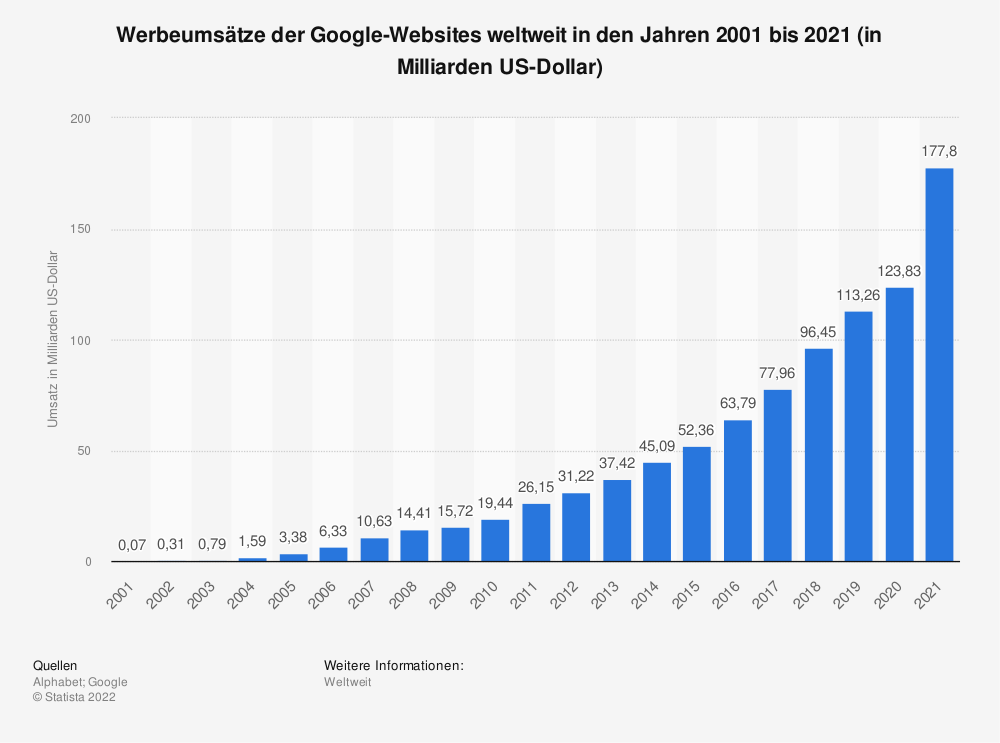
\includegraphics[width=.8\textwidth]{figures/appendix/werbeumsatz.png}
    \caption{Werbeumsätze Google Websites \cite{alphabet2022}}
    \label{fig:werbeumsatz}
  \end{centering}
\end{wrapfigure}

\begin{wrapfigure}{r}{\textwidth}
  \begin{centering}
    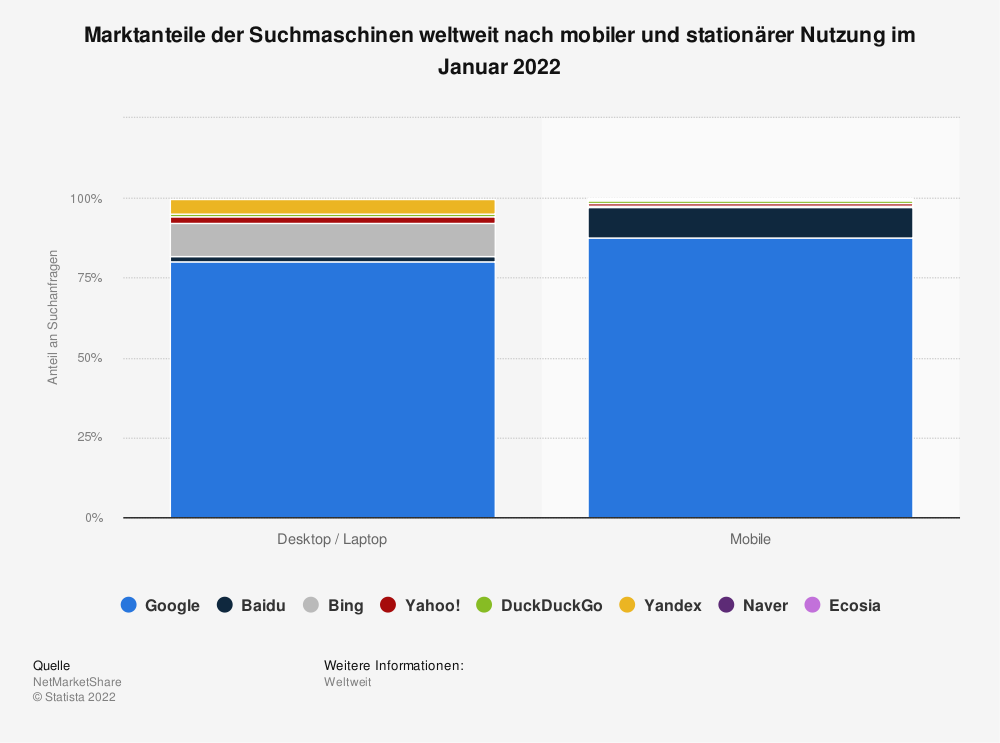
\includegraphics[width=.8\textwidth]{figures/appendix/marketshare.png}
    \caption{Marktanteil Google \cite{netmarketshare2022}}
    \label{fig:marketshare}
  \end{centering}
\end{wrapfigure}

\begin{wrapfigure}{r}{\textwidth}
  \begin{centering}
    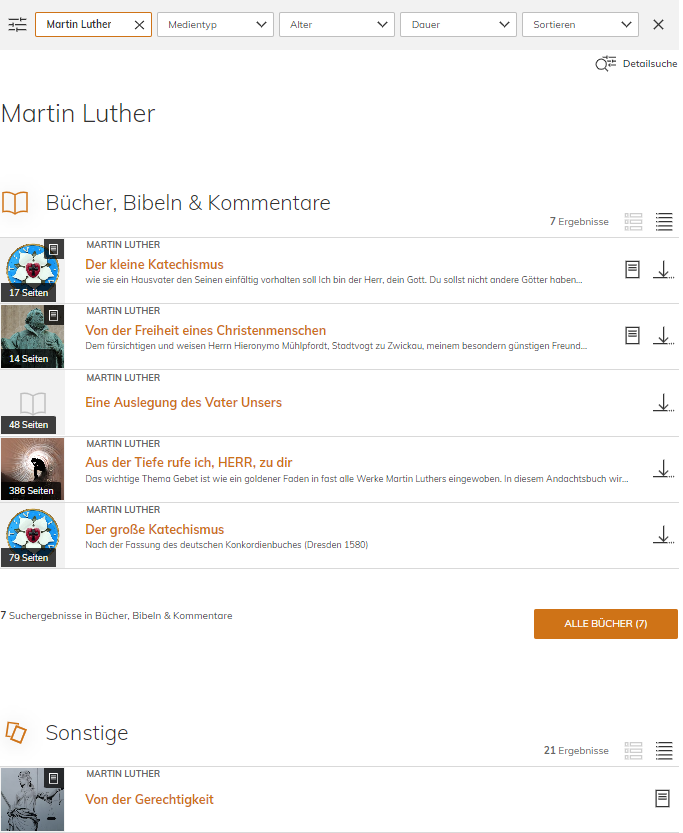
\includegraphics[width=.8\textwidth]{figures/appendix/crossloadSuche.png}
    \caption{Crossload \cite{pfleiderer2022}}
    \label{fig:crossloadSuche}
  \end{centering}
\end{wrapfigure}


% 2 Images on one page
% \begin{figure}
%   \includegraphics[width=\textwidth]{figures/appendix/IMAGE.png}
%   \caption{\label{fig:IMAGE} TITLE \cite{CITATION}}
%   \includegraphics[width=\textwidth]{figures/appendix/IMAGE.png}
%   \caption{\label{fig:IMAGE} TITLE \cite{CITATION}}
% \end{figure}

% 1 Images per page
% \begin{figure}
%   \includegraphics[width=\textwidth]{figures/appendix/IMAGE.png}
%   \caption{\label{fig:IMAGE} TITLE \cite{CITATION}}
% \begin{figure}
% \end{figure}
%   \includegraphics[width=\textwidth]{figures/appendix/IMAGE.png}
%   \caption{\label{fig:IMAGE} TITLE \cite{CITATION}}
% \end{figure}

\backmatter
\listoffigures
\listoftables
\bibliographystyle{ieeetr}
\bibliography{refs}

\end{document}
